% ====================================================================
\section{Composition: the serial tree processor}\label{sec:processor}
% ====================================================================

Fix an MSLP $\mathcal P$ in normal form with registers $R_1,\dots,R_m$. For an instruction register
$k$ we write $i=i_k$, $j=j_k$ (so $i,j<k$) and $\circ_k$, and we say that $k$ has
\emph{background} $c_k=0$ if $\circ_k=\wedge$ and $c_k=1$ if $\circ_k=\vee$. The last instruction
is an $\AND$, so $c_m=0$.

\subsection{The physical processor}\label{sec:physical}

\begin{definition}[Processor]\label{def:processor}
The processor $P(m)$ is the cell network with:
\begin{itemize}
\item cells $E_0,\dots,E_m$ (the \emph{bus}); for each $1\le i\le m$, cells $C_i$ (front isolator),
  $K_i$ (buffer) and $R_i$ (register); and the cells $F_A,K_A,Q_A,F_B,K_B,Q_B$ (two \emph{fronts},
  two buffers and two \emph{temporaries});
\item junctions $G$ and $r_1,\dots,r_m$, each with its control $h_G$ or $h_i=h_{r_i}$;
\item external ports, called \emph{far clocks}: $\kappa_1,\dots,\kappa_m,\kappa_A,\kappa_B,\kend$;
\end{itemize}
connected at the cell level as follows, where each dash is one edge between endpoints or between an
endpoint and a junction or port:
\begin{gather*}
G\;-\;E_0\;-\;r_1\;-\;E_1\;-\;r_2\;-\;\cdots\;-\;r_m\;-\;E_m\;-\;\kend,\\
r_i\;-\;C_i\;-\;K_i\;-\;R_i\;-\;\kappa_i\quad(1\le i\le m),\\
G\;-\;F_X\;-\;K_X\;-\;Q_X\;-\;\kappa_X\quad(X\in\{A,B\}).
\end{gather*}
Each endpoint has its two control slots and each junction its control slot $h$. The far clocks are
also control slots: their consumers are the endpoints $\ep{R_i}{\kappa_i}$, $\ep{Q_X}{\kappa_X}$ and
$\ep{E_m}{\kend}$.
\end{definition}

\begin{figure}[ht]
\centering
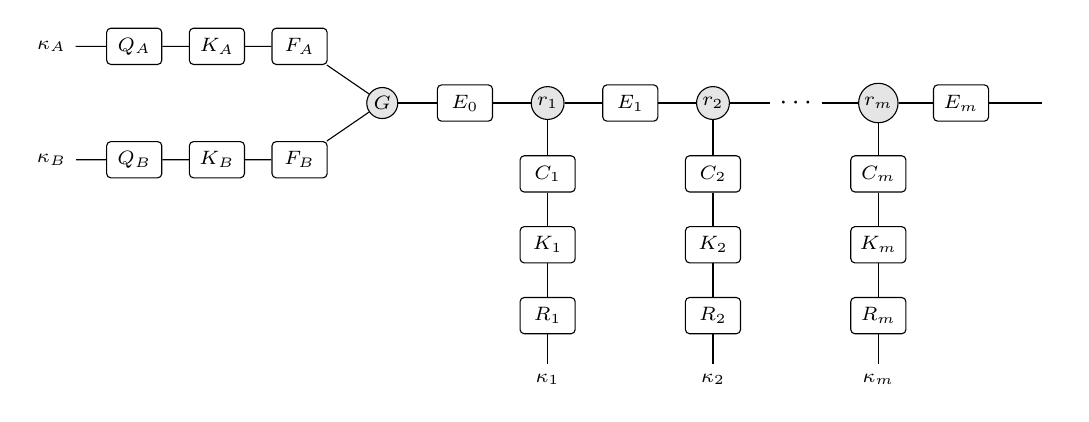
\begin{tikzpicture}[x=1.05cm,y=0.9cm,
  cell/.style={draw,rounded corners=1.5pt,minimum width=7mm,minimum height=4.6mm,font=\scriptsize,inner sep=1pt},
  jn/.style={circle,draw,fill=black!10,inner sep=1.2pt,font=\scriptsize},
  port/.style={font=\scriptsize}]
\node[jn] (G) at (0,0) {$G$};
\node[cell] (E0) at (1,0) {$E_0$};
\node[jn] (r1) at (2,0) {$r_1$};
\node[cell] (E1) at (3,0) {$E_1$};
\node[jn] (r2) at (4,0) {$r_2$};
\node (dots) at (5,0) {$\cdots$};
\node[jn] (rm) at (6,0) {$r_m$};
\node[cell] (Em) at (7,0) {$E_m$};
\node[port] (ke) at (8.1,0) {$\kend$};
\foreach \r/\x/\i in {r1/2/1,r2/4/2,rm/6/m}{
  \node[cell] (C\i) at (\x,-1) {$C_{\i}$};
  \node[cell] (K\i) at (\x,-2) {$K_{\i}$};
  \node[cell] (R\i) at (\x,-3) {$R_{\i}$};
  \node[port] (k\i) at (\x,-3.9) {$\kappa_{\i}$};
  \draw (\r)--(C\i)--(K\i)--(R\i)--(k\i);
}
\node[cell] (FA) at (-1,0.8) {$F_A$}; \node[cell] (KA) at (-2,0.8) {$K_A$};
\node[cell] (QA) at (-3,0.8) {$Q_A$}; \node[port] (kA) at (-4,0.8) {$\kappa_A$};
\node[cell] (FB) at (-1,-0.8) {$F_B$}; \node[cell] (KB) at (-2,-0.8) {$K_B$};
\node[cell] (QB) at (-3,-0.8) {$Q_B$}; \node[port] (kB) at (-4,-0.8) {$\kappa_B$};
\draw (G)--(E0)--(r1)--(E1)--(r2)--(dots)--(rm)--(Em)--(ke);
\draw (G)--(FA)--(KA)--(QA)--(kA);
\draw (G)--(FB)--(KB)--(QB)--(kB);
\end{tikzpicture}
\caption{The processor at the cell level. Each box is a two-vertex cell, each circle a junction.
Control slots are not drawn: two per cell endpoint and one per junction.}
\label{fig:processor}
\end{figure}

\begin{lemma}[Topology]\label{lem:proctopology}
$P(m)$ is a tree. Every cell endpoint and every junction has degree exactly four, and every control
slot, far clocks included, is a leaf.
\end{lemma}

\begin{proof}
At the cell level the network is a path ($G$, the bus, $\kend$) with pendant paths (the register
arms, the two temporary arms, and the far clocks). This is a tree. Each cell is an edge, each cell
adjacency is realised by exactly one edge, and the control slots are leaves. Replacing nodes of a
tree by subtrees joined through single edges gives a tree. An endpoint has its partner, one data
port (a junction, an endpoint of an adjacent cell, or a far clock) and two control slots. A
junction has three arms and one control.
\end{proof}

\begin{definition}[Phase assignment]\label{def:procphases}
Cells $E_i,C_i,R_i,F_X,Q_X$ have phase $0$; buffers $K_i,K_X$ have phase $1$; every junction control
has phase $1$; every far clock has phase $0$.
\end{definition}

This is the two-colouring of the cell-level tree, with junction controls placed on the colour
opposite to their arms. The arms of every junction have phase $0$ and its control has phase $1$.
Adjacent cells in the chains $C_i\,$--$\,K_i\,$--$\,R_i$ and $F_X\,$--$\,K_X\,$--$\,Q_X$ have opposite
phases. These are exactly the local conventions of \cref{tab:timing}, with $e=0$ for junction arms
and for the cells $A,B,C,R$ of a read, and $e\oplus1=1$ for buffers and junction controls.

\subsection{Normal configurations}

\begin{definition}[Normal configuration]\label{def:normal}
For $c\in\{0,1\}$ and $\rho:[1,m]\to\{0,1\}$, the configuration $\NORMAL(c,\rho)$ is:
\begin{itemize}
\item every bus cell $E_i=cc$, and $x_G=x_{r_i}=c$ for all $i$;
\item $C_i=K_i=bb$ and $R_i=\rho(i)\rho(i)$ for all $i$;
\item $F_A=K_A=Q_A=F_B=K_B=Q_B=bb$; the temporaries are \emph{free}.
\end{itemize}
The \emph{rest schedule of background $c$} puts every cell in \HOLD, every junction control at $c$,
and every far clock at $b$.
\end{definition}

\begin{lemma}[Stability]\label{lem:normalstable}
$\NORMAL(c,\rho)$ is a fixed point of the forced evolution under the rest schedule of background $c$.
\end{lemma}

\begin{proof}
All cells are uniform and in \HOLD\ (\cref{lem:frame}\ref{frame:hold}). The arms of $r_i$ are
$E_{i-1}=c$, $E_i=c$ and $C_i=b$, so one of them is $b$. The arms of $G$ are $E_0=c$, $F_A=b$ and
$F_B=b$, so two of them are $b$. Apply \cref{lem:frame}\ref{frame:junction}.
\end{proof}

The initial configuration of the processor is $\NORMAL(0,\rho_0)$, where $\rho_0(i)=\iota_0(i)$ for
input registers and $\rho_0(k)=0$ for instruction registers.

\subsection{One instruction}\label{sec:instruction}

Fix an instruction register $k$. Let $c=c_k$ be its background, $b=1-c$, $x=\rho(i)$,
$y=\rho(j)$, $d=x\circ_k y$, and $\rho'=\rho[k\mapsto d]$. The \emph{instruction schedule}
$\Sigma_k$ consists of the twelve phases of \cref{tab:instruction}, executed in order. Each phase
starts at the first time, not earlier than the end of the previous phase, whose parity equals the
phase's reference parity. The resulting idle step, when present, is called an \emph{alignment
wait}: it uses the rest schedule.

\begin{table}[ht]
\centering\small
\begin{tabular}{r>{\raggedright\arraybackslash}p{8.4cm}cc}\toprule
& phase (primitives, in order; $\parallel$ = simultaneous) & duration & ref.\ parity\\\midrule
1 & \prim{PREPARE}: $\prim{SET}(C_k\mathbin{:=}c)$; then $\prim{SET}(K_k\mathbin{:=}c)\parallel\prim{SET}(R_k\mathbin{:=}b)$ & $6$ & $c$\\
2 & $\prim{FETCH}(i,F_A)$ (\cref{lem:fetch}) & $12i+18$ & $c$\\
3 & \prim{STORE}: $\prim{SET}(K_A\mathbin{:=}b)$; $\prim{MOVE}_b(F_A\to K_A)$; $\prim{MOVE}_b(K_A\to Q_A)$ & $9$ & $c$\\
4 & $\prim{FETCH}(j,F_B)$ & $12j+18$ & $c$\\
5 & \prim{RECOVER}: $\prim{COPY}$ $Q_A\to K_A$ via $\FAV c$; $\prim{SET}(F_A\mathbin{:=}c)$; $\prim{MOVE}_c(K_A\to F_A)$ & $9$ & $1\oplus c$\\
6 & $\prim{GATE}_c(G;F_A,F_B\to E_0)$ & $5$ & $1\oplus c$\\
7 & \prim{CLEAN}: $\prim{SET}(Q_A\mathbin{:=}b)\parallel\prim{SET}(Q_B\mathbin{:=}b)$; then $\prim{SET}(K_A\mathbin{:=}b)\parallel\prim{SET}(K_B\mathbin{:=}b)$ & $6$ & $1\oplus c$\\
8 & \prim{LEFT}: transport $E_0\to E_{k-1}$ through $r_1,\dots,r_{k-1}$ (\cref{lem:chain}) & $6(k-1)$ & $c$\\
9 & \prim{PILOT}: $\prim{COPY}$ $\kend\to E_m$ via $\FAV b$ & $3$ & $1\oplus c$\\
10 & \prim{RIGHT}: transport $E_m\to E_k$ through $r_m,\dots,r_{k+1}$ & $6(m-k)$ & $c$\\
11 & \prim{COMMIT}: $\prim{ROUTE}(r_k;E_{k-1}\to C_k;E_k)$; $\prim{SET}(K_k\mathbin{:=}b)$; $\prim{MOVE}_b(C_k\to K_k)$; $\prim{MOVE}_b(K_k\to R_k)\parallel\prim{SET}(E_k\mathbin{:=}c)$ & $15$ & $c$\\
12 & \prim{FRONTS}: $\prim{SET}(F_A\mathbin{:=}b)\parallel\prim{SET}(F_B\mathbin{:=}b)$ & $3$ & $1\oplus c$\\\bottomrule
\end{tabular}
\caption{The instruction schedule $\Sigma_k$, for background $c=c_k$.}
\label{tab:instruction}
\end{table}

\begin{lemma}[Admissibility and alignment of $\Sigma_k$]\label{lem:sigmatiming}
With the phase assignment of \cref{def:procphases}, every block and control event of every phase of
\cref{tab:instruction} is admissible when the phase starts at its reference parity. If $\Sigma_k$
starts at a time $S\equiv c$, alignment waits occur exactly before phases $4$, $5$, $6$, $7$, $8$
and $9$, one transition each. The schedule ends at $S+D_k$ with
\[
D_k=12(i+j)+6m+92,
\]
which is even, so it ends at parity $c$.
\end{lemma}

\begin{proof}
We use \eqref{eq:startparity}, writing each event as (phase, $\zeta$, offset).
\begin{itemize}
\item Phase 1: $C_k$ $(0,0,0)$; $K_k$ $(1,0,3)$; $R_k$ $(0,1,3)$. All give $c$.
\item Phases 2 and 4: by \cref{lem:fetch} below.
\item Phase 3: $K_A$ $(1,1,0)$; $\prim{MOVE}_b(F_A\to K_A)$ $(0,1,3)$; $\prim{MOVE}_b(K_A\to Q_A)$
  $(1,1,6)$. All give $c$.
\item Phase 5: $K_A$ in $\FAV c$ $(1,0,0)$; $F_A$ $(0,0,3)$; $\prim{MOVE}_c(K_A\to F_A)$ $(1,0,6)$. All
  give $1\oplus c$.
\item Phase 6: \cref{tab:timing} with $e=0$ gives $1\oplus c$.
\item Phase 7: $Q$'s $(0,1,0)$; $K$'s $(1,1,3)$. Both give $1\oplus c$.
\item Phases 8 and 10: routes with $e=0$, at even offsets, give $c$.
\item Phase 9: $E_m$ $(0,1,0)$ gives $1\oplus c$.
\item Phase 11: route $(e=0)$ at offset $0$ gives $c$; $K_k$ $(1,1,6)$; $\prim{MOVE}_b(C_k\to K_k)$
  $(0,1,9)$; $\prim{MOVE}_b(K_k\to R_k)$ $(1,1,12)$; $E_k$ $(0,0,12)$. All give $c$.
\item Phase 12: $(0,1,0)$ gives $1\oplus c$.
\end{itemize}
Durations are $6$, even, $9$, even, $9$, $5$, $6$, even, $3$, even, $15$, $3$. Starting at parity
$c$, the end parities are $c,c,1{\oplus}c,c,c,c,1{\oplus}c,c,c,c,1{\oplus}c,c$. Comparing each end
parity with the next phase's reference parity gives one wait before phases $4,5,6,7,8,9$ and none
elsewhere. Summing,
$6+(12i+18)+9+1+(12j+18)+1+9+1+5+1+6+1+6(k-1)+1+3+6(m-k)+15+3=12(i+j)+6m+92$.
\end{proof}

\paragraph{Milestones.} \Cref{tab:milestones} lists the configuration at the end of each phase as a
difference from $\NORMAL(c,\rho)$. At every milestone all cells are uniform and in \HOLD, all
junctions are in state $c$, and all controls are at rest. In the proofs, ``$M_r$ plus $X=uu$'' means
the milestone $M_r$ with the cell $X$ replaced.

\begin{table}[ht]
\centering\small
\begin{tabular}{cl}\toprule
milestone & differences from $\NORMAL(c,\rho)$\\\midrule
$M_0$ & none\\
$M_1$ & $C_k=K_k=cc$, $R_k=bb$\\
$M_2$ & $M_1$ plus $F_A=xx$, $K_A=cc$\\
$M_3$ & $M_1$ plus $Q_A=xx$\\
$M_4$ & $M_3$ plus $F_B=yy$, $K_B=cc$\\
$M_5$ & $M_1$ plus $F_A=xx$, $K_A=cc$, $Q_A=xx$, $F_B=yy$, $K_B=cc$\\
$M_6$ & $M_1$ plus $F_A=F_B=cc$, $K_A=K_B=cc$, $Q_A=xx$, $E_0=dd$\\
$M_7$ & $M_1$ plus $F_A=F_B=cc$, $E_0=dd$\\
$M_8$ & $M_1$ plus $F_A=F_B=cc$, $E_{k-1}=dd$\\
$M_9$ & $M_8$ plus $E_m=bb$\\
$M_{10}$ & $M_8$ plus $E_k=bb$\\
$M_{11}$ & $\NORMAL(c,\rho')$ plus $F_A=F_B=cc$\\
$M_{12}$ & $\NORMAL(c,\rho')$\\\bottomrule
\end{tabular}
\caption{Milestones of $\Sigma_k$: $M_r$ is the configuration at the end of phase $r$.}
\label{tab:milestones}
\end{table}

\begin{lemma}[Alignment waits]\label{lem:waits}
Every milestone $M_r$, $0\le r\le 12$, is a fixed point of the forced evolution under the rest
schedule of background $c$. Hence the alignment waits do not change the configuration.
\end{lemma}

\begin{proof}
All cells are uniform and in \HOLD. By \cref{lem:frame} it suffices that every junction has at
most two arms in state $b$ (arms read as their adjacent endpoints).
\begin{itemize}
\item $G$, arms $(E_0,F_A,F_B)$: $(c,b,b)$ in $M_0,M_1,M_3,M_{12}$; $(c,x,b)$ in $M_2$; $(c,b,y)$
  in $M_4$; $(c,x,y)$ in $M_5$; $(d,c,c)$ in $M_6,M_7$; $(c,c,c)$ in $M_8$--$M_{11}$.
\item $r_k$: in $M_1$--$M_{10}$ its arm $C_k$ is $c$, so at most its two bus arms are $b$. In $M_0$,
  $M_{11}$ and $M_{12}$, its bus arms are $c$.
\item $r_\ell$, $\ell\ne k$: its arm $C_\ell$ is $b$, and in every milestone at most one of
  $E_{\ell-1},E_\ell$ differs from $c$. The only milestone with two non-background bus cells is
  $M_{10}$, where they are $E_{k-1}$ and $E_k$, both arms of $r_k$; and $M_9$ with $k<m$, where
  they are $E_{k-1}$ and $E_m$, which are not arms of a common junction because $k-1<m-1$.\qedhere
\end{itemize}
\end{proof}

\begin{lemma}[\prim{PREPARE}: $M_0\to M_1$]\label{lem:prepare}
Starting from $M_0$, phase~1 produces $M_1$.
\end{lemma}

\begin{proof}
During $[s,s+3)$, $C_k$ is in $\FAV c$ and its port $x_{r_k}$ is $c$ at control time $s$. The
junction $r_k$ stays $c$, since its arms are $E_{k-1}=E_k=c$ and $C_k$. By \cref{lem:forcing},
$C_k=cc$ at $s+2$ and $s+3$. During $[s+3,s+6)$, $K_k$ is in $\FAV c$ with port $\ep{C_k}{K_k}=c$ at
control time $s+3$, and $R_k$ is in $\FAV b$ with port $\kappa_k=b$. By \cref{lem:forcing}, at $s+6$
we have $K_k=cc$ and $R_k=bb$. No other cell changes.
\end{proof}

Only a fresh destination is overwritten this way: $R_k$ has not been read before instruction $k$,
and it is never read before it is written. Inputs and earlier results are never prepared.

\begin{lemma}[\prim{FETCH}]\label{lem:fetch}
Let $1\le i\le m$, let $F\in\{F_A,F_B\}$ with buffer $K_F$ and temporary $Q_F$, and let $F'$ be the
other front. Assume that at time $s$, with $s\equiv c$, all cells are uniform and in \HOLD, all
controls are at rest, and:
\begin{enumerate}[label=(\alph*)]
\item every bus cell is $cc$ and every junction is in state $c$;
\item $C_\ell=K_\ell=bb$ for all $\ell\le i$, and $R_i=xx$;
\item $F=K_F=Q_F=bb$ and $F'=bb$. The cells $K_{F'}$ and $Q_{F'}$ are arbitrary uniform cells; they
  may hold a protected value.
\end{enumerate}
Apply the schedule
\begin{center}\small
\begin{tabular}{ll}\toprule
control times & operation\\\midrule
$[s,s+6)$ & $\prim{ROUTE}(G;F\to E_0;F')$ (emit a pilot $b$)\\
$s+6$ & wait\\
$[s+7,s+10)$ & $\prim{SET}(K_F\mathbin{:=}c)$ from $F=c$\\
$[s+10,s+4+6i)$ & transport $E_0\to E_{i-1}$ through $r_1,\dots,r_{i-1}$\\
$[s+4+6i,s+18+6i)$ & $\prim{READ}(r_i;E_{i-1};C_i,K_i,R_i)$\\
$[s+18+6i,s+12+12i)$ & transport $E_{i-1}\to E_0$ through $r_{i-1},\dots,r_1$\\
$[s+12+12i,s+18+12i)$ & $\prim{ROUTE}(G;E_0\to F;F')$\\\bottomrule
\end{tabular}
\end{center}
Then at time $s+12i+18$ the configuration equals the initial one, except that $F=xx$ and
$K_F=cc$. All blocks and control events are admissible, with reference parity $c$.
\end{lemma}

\begin{proof}
Admissibility: the routes and the read have reference parity $c$ (\cref{tab:timing}, $e=0$) and
start at even offsets $0$, $10+6\ell$, $4+6i$, $18+6i+6\ell$ and $12+12i$. The block of
$\prim{SET}(K_F\mathbin{:=}c)$ is $(1,0,7)$, which also gives $c$.

\emph{Emit.} The route at $G$ has source $F=bb$, destination $E_0=cc$ and bias $F'=bb$, with
$x_G=c$. The far port of $E_0$ is $r_1$. Its arms are $E_0$, $E_1=c$ and $C_1=b$, so it stays $c$ by
the frame lemma. \Cref{lem:route} gives $F=cc$, $E_0=bb$ (the pilot) and $x_G=c$ at $s+6$.

\emph{Wait.} The configuration at $s+6$ is stable: $G$ has arms $(E_0,F,F')=(b,c,b)$, and $r_1$ has
arms $(b,c,b)$.

\emph{Buffer.} $K_F$ is in $\FAV c$ during $[s+7,s+10)$, and its port $\ep F{K_F}$ is $c$, so
\cref{lem:forcing} gives $K_F=cc$. $Q_F=bb$ is untouched.

\emph{Outward transport.} Apply \cref{lem:chain} with $X_0=E_0$ (carrying $b$), junctions
$r_1,\dots,r_{i-1}$, cells $E_1,\dots,E_{i-1}$ and biases $C_1,\dots,C_{i-1}=bb$. The final far port is
$r_i$, whose arms are $E_{i-1}$, $E_i=c$ and $C_i=b$, so it stays $c$. The vertex beyond $X_0$ is $G$,
whose arms are $E_0$, $F=c$ and $F'=b$, so it stays $c$. For $i=1$ this step is empty and the pilot
stays in $E_0$.

\emph{Read.} At time $s+4+6i$, the cells $A=E_{i-1}=bb$ (pilot), $B=E_i=cc$, $C=C_i=bb$, $K=K_i=bb$
and $R=R_i=xx$ satisfy the hypotheses of \cref{lem:read} at $g=r_i$. The far port of $A$ is $r_{i-1}$,
or $G$ if $i=1$, and it stays $c$ throughout the read. The arms of $r_{i-1}$ are $E_{i-2}=c$,
$C_{i-1}=b$ and $E_{i-1}$. The arms of $G$ are $E_0$, $F=c$ and $F'=b$. The far ports of $B$ and $R$
are irrelevant. All other junctions have unchanged arms. The read returns $E_{i-1}=xx$, $r_i=c$,
$C_i=K_i=bb$, $R_i=xx$ and $E_i=cc$.

\emph{Return transport.} Apply \cref{lem:chain} with $X_0=E_{i-1}$, with junctions
$r_{i-1},\dots,r_1$, cells $E_{i-2},\dots,E_0$ and biases $C_{i-1},\dots,C_1=bb$. The final far port is $G$, which stays
$c$ by the frame lemma, because its arms are $E_0$, $F=c$ and $F'=b$. The vertex beyond $X_0$ is
$r_i$, whose arms are $E_{i-1}$, $E_i=c$ and $C_i=b$.

\emph{Deliver.} The route at $G$ has source $E_0=xx$, destination $F=cc$ and bias $F'=bb$. The
destination's far port is $\ep{K_F}{F}=c$. The source's far port $r_1$ is arbitrary for the route;
its arms are $E_0$, $E_1=c$ and $C_1=b$, so it stays $c$. The result is $F=xx$ and $E_0=cc$.
\end{proof}

All register arms that were visited return to their normal state. The cases $i=1$ (empty transports)
and $F=F_B$ with $Q_A$ holding a value (condition (c)) are covered.

\begin{lemma}[\prim{STORE}: $M_2\to M_3$]\label{lem:store}
Starting from $M_2$, phase 3 produces $M_3$.
\end{lemma}

\begin{proof}
$\prim{SET}(K_A\mathbin{:=}b)$: its port $\ep{Q_A}{K_A}=b$ forces $K_A=bb$ (\cref{lem:forcing}), while
$F_A=xx$ is in \HOLD. Then $\prim{MOVE}_b(F_A\to K_A)$: the destination is $K_A=bb$ and its far port
is $\ep{Q_A}{K_A}=b$; the source's far port $G$ is arbitrary. \Cref{lem:move} gives $F_A=bb$ and
$K_A=xx$. Then $\prim{MOVE}_b(K_A\to Q_A)$: the destination is $Q_A=bb$ with far port $\kappa_A=b$,
giving $K_A=bb$ and $Q_A=xx$. Throughout, $G$ has $x_G=h_G=c$ and arm $E_0=c$, so it keeps $c$. The
known bit $b$ is left in front of the stored operand.
\end{proof}

At $M_3$ the front $F_A$ is $b$ and $Q_A$ holds $x$. The second fetch then runs with
$F=F_B$ and $F'=F_A=bb$, and condition (c) of \cref{lem:fetch} holds. In particular, there is no
attempt to restore $F_A$ while a pilot is in $E_0$.

\begin{lemma}[\prim{RECOVER}: $M_4\to M_5$]\label{lem:recover}
Starting from $M_4$, phase 5 produces $M_5$.
\end{lemma}

\begin{proof}
\emph{Copy.} $K_A=bb$ is in $\FAV c$. Its port on the $Q_A$ side is constantly $x$, because $Q_A$ is
in \HOLD, and its port on the $F_A$ side is constantly $b$, because $F_A=bb$ is in \HOLD. The dual form
of \cref{lem:copy} gives $K_A=xx$, and $Q_A$ is unchanged.
\emph{Clear the front.} $F_A$ is in $\FAV c$ with port $x_G=c$, so $F_A=cc$ (\cref{lem:forcing}).
\emph{Move back.} $\prim{MOVE}_c(K_A\to F_A)$: the destination is $F_A=cc$ and its far port is $x_G$;
the source's far port $Q_A$ is arbitrary. This gives $K_A=cc$ and $F_A=xx$.
During the whole phase, $x_G$, $h_G$ and the arm $E_0$ are all $c$, so $x_G=c$ is an invariant, not
an assumption about the port.
\end{proof}

\begin{lemma}[Gate step: $M_5\to M_6$]\label{lem:gatestep}
Starting from $M_5$, phase 6 produces $M_6$, with $E_0=dd$ and $d=x\circ_k y$.
\end{lemma}

\begin{proof}
Apply \cref{lem:gate} at $G$ with $A=F_A=xx$, $B=F_B=yy$ and $C=E_0=cc$. The far port of $E_0$ is
$r_1$, whose arms are $E_0$, $E_1=c$ and $C_1=b$; $C_1=b$ because $k\ge2$. So $r_1$ stays $c$. The
operands' far ports $K_A$, $K_B$ are arbitrary. The result has $E_0=dd$ and $F_A=F_B=cc$. The result
is already on the bus, so no third temporary is needed.
\end{proof}

\begin{lemma}[\prim{CLEAN}: $M_6\to M_7$]\label{lem:clean}
Starting from $M_6$, phase 7 produces $M_7$.
\end{lemma}

\begin{proof}
$Q_A$ and $Q_B$ are forced to $bb$ through their far clocks, which are $b$; then $K_A$ and $K_B$ are
forced to $bb$ through $\ep{Q_X}{K_X}=b$ (\cref{lem:forcing}). These cells are not arms of $G$, and $G$
keeps $c$ because $F_A=F_B=c$.
\end{proof}

\begin{remark}[Why the fronts stay at $c$]\label{rem:fronts}
While $E_0$ holds $d$, the fronts must remain $c$. If $d=b$ and both fronts were restored to $b$, then
$G$ would have three arms in state $b$ and would flip. Restoring the buffers and temporaries early is
harmless, because they are not arms of $G$. The fronts are restored in phase 12, after $E_0=c$.
\end{remark}

\begin{lemma}[Writing routes: $M_7\to M_{10}$]\label{lem:writeroutes}
Starting from $M_7$, phases 8, 9 and 10 produce $M_8$, $M_9$ and $M_{10}$ in turn. Throughout, the
packets stay on opposite sides of $r_k$ and never cross it.
\end{lemma}

\begin{proof}
\emph{Left.} Apply \cref{lem:chain} with $X_0=E_0$ (carrying $d$), junctions $r_1,\dots,r_{k-1}$ and
biases $C_1,\dots,C_{k-1}=bb$. Every traversed arm has bias $b$, including the arms read in phases 2
and 4: since $i,j<k$, the prepared arm $C_k=c$ is not traversed. The final far port is $r_k$, whose
arms are $E_{k-1}$, $E_k=c$ and $C_k=c$, so it stays $c$ even if $d=b$. The vertex beyond $X_0$ is
$G$, whose arms are $F_A=F_B=c$, so it stays $c$.

\emph{Pilot.} $E_m=cc$ is in $\FAV b$, with port $\kend=b$ constant and other port $x_{r_m}$. The
junction $r_m$ stays $c$. If $k=m$, its arms are $E_{m-1}=d$, $C_m=c$ and $E_m$. If $k<m$, its arms
are $E_{m-1}=c$, $C_m=b$ and $E_m$. By \cref{lem:copy}, $E_m=bb$.

\emph{Right.} If $k<m$, apply \cref{lem:chain} with $X_0=E_m$ (carrying $b$), junctions
$r_m,\dots,r_{k+1}$, cells $E_{m-1},\dots,E_k=cc$ and biases $C_m,\dots,C_{k+1}=bb$. The final far port
is $r_k$, whose arms are $E_{k-1}=d$, $C_k=c$ and $E_k$, so it stays $c$. Beyond $X_0$ is the
external port $\kend$. If $k=m$ the phase is empty and $M_9=M_{10}$.

While both packets wait next to $r_k$, the arm $C_k=c$ keeps $r_k$ at $c$ even when $d=b$. Leaving
$C_k=b$ would not have this property; this is why the destination is prepared before the fetches.
\end{proof}

\begin{lemma}[\prim{COMMIT}: $M_{10}\to M_{11}$]\label{lem:commit}
Starting from $M_{10}$ at time $s$, phase 11 produces $M_{11}$ at $s+15$: $E_{k-1}=E_k=cc$,
$C_k=K_k=bb$, $R_k=dd$ and $x_{r_k}=c$.
\end{lemma}

\begin{proof}
\emph{$[s,s+6)$: route.} \Cref{lem:route} at $r_k$, with source $E_{k-1}=dd$, destination $C_k=cc$,
bias $E_k=bb$ and $x_{r_k}=c$. The destination's far port is $\ep{K_k}{C_k}=c$. The source's far port
is $r_{k-1}$ (which exists because $k\ge 2$); its arms are $E_{k-2}=c$, $C_{k-1}=b$ and
$E_{k-1}$, so it stays $c$. Result: $C_k=dd$, $E_{k-1}=cc$.

\emph{$[s+6,s+9)$: buffer.} $K_k$ is in $\FAV b$, with port $\ep{R_k}{K_k}=b$, so $K_k=bb$. The
junction $r_k$ has arms $E_{k-1}=c$, $E_k=b$ and $C_k=d$, so it stays $c$.

\emph{$[s+9,s+12)$: first move.} $\prim{MOVE}_b(C_k\to K_k)$: the destination is $K_k=bb$ and its far
port is $\ep{R_k}{K_k}=b$; the source's far port $r_k$ is arbitrary. Result: $C_k=bb$ and $K_k=dd$.
The isolator $C_k$ is restored while the datum advances. The junction $r_k$ keeps $c$, because
$x_{r_k}$, $h_k$ and $E_{k-1}$ are $c$.

\emph{$[s+12,s+15)$: second move and pilot erasure.} $\prim{MOVE}_b(K_k\to R_k)$: the destination is
$R_k=bb$ and its far port is $\kappa_k=b$. Result: $K_k=bb$ and $R_k=dd$. Simultaneously $E_k$ is in
$\FAV c$ with port $x_{r_k}=c$, so $E_k=cc$; its other port, $r_{k+1}$ or $\kend$ when $k=m$, may be
arbitrary. During erasure, $x_{r_k}$, $h_k$ and $E_{k-1}$ are all $c$, so even $C_k=E_k=b$ cannot flip
$r_k$. If $k<m$, the junction $r_{k+1}$ has arms $E_k$, $E_{k+1}=c$ and $C_{k+1}=b$, so it stays $c$.
\end{proof}

Restoration happens \emph{during} transport: the first move restores $C_k$ while advancing the
datum, and the second restores $K_k$ while writing $R_k$. It does not happen after a uniform
channel has joined two equal stored values.

\begin{lemma}[\prim{FRONTS}: $M_{11}\to M_{12}$]\label{lem:fronts}
Starting from $M_{11}$, phase 12 produces $M_{12}$, which is $\NORMAL(c,\rho')$.
\end{lemma}

\begin{proof}
$F_A$ and $F_B$ are forced to $bb$ through $\ep{K_X}{F_X}=b$. The junction $G$ keeps $c$, because
$x_G$, $h_G$ and $E_0$ are $c$.
\end{proof}

\begin{proposition}[Instruction step]\label{prop:instruction}
Let $k$ be an instruction register and $c=c_k$. If the processor is in $\NORMAL(c,\rho)$ at a time
$S\equiv c$ and $\Sigma_k$ is applied from $S$, then it is in $\NORMAL(c,\rho[k\mapsto
\rho(i)\circ_k\rho(j)])$ at time $S+D_k$, where $D_k=12(i+j)+6m+92$. All blocks and control events
of $\Sigma_k$ are admissible. The schedule $\Sigma_k$ depends only on $k$, $i$, $j$ and $\circ_k$,
not on $\rho$.
\end{proposition}

\begin{proof}
Chain \cref{lem:prepare,lem:fetch,lem:store,lem:recover,lem:gatestep,lem:clean,lem:writeroutes,lem:commit,lem:fronts},
with the waits justified by \cref{lem:waits} and the timing by \cref{lem:sigmatiming}. The fetch
lemma applies in phase 2 at $M_1$: $C_\ell=K_\ell=bb$ for $\ell\le i$ because $k>i$. It applies in
phase 4 at $M_3$ because $k>j$, $F_B=K_B=Q_B=bb$ and $F_A=bb$. When $i=j$, the first read restored
$C_i$, $K_i$ and $R_i$ before the second read. No step consults the bits $x$, $y$ or $d$.
\end{proof}

\subsection{Changing the background}\label{sec:normalize}

\begin{lemma}[\prim{NORMALIZE}]\label{lem:normalize}
Suppose the processor is in $\NORMAL(c,\rho)$ at a time $s_0\equiv c$. Put $t_0=s_0+6$,
$t_j=t_0+4(m-j)$ for $1\le j\le m$, and $s=t_0+4m$. Apply:
\begin{center}\small
\begin{tabular}{ll}\toprule
control times & modes and controls\\\midrule
$[s_0,s_0+3)$ & $\prim{SET}(F_A\mathbin{:=}c)$\\
$[s_0+3,t_0)$ & $\prim{COPY}$ $\kend\to E_m$ via $\FAV b$\\
from $t_0$ on & every far clock changes from $b$ to $c$\\
$[t_j,t_j+3)$ & $C_j$ in $\FAV c$; $h_j$ changes from $c$ to $b$ at $t_j$ and stays $b$\\
$[t_j+1,t_j+4)$ & $K_j$ in $\FAV c$, $E_{j-1}$ in $\FAV b$\\
$[s,s+3)$ & $F_A,F_B,Q_A,Q_B$ in $\FAV c$; $h_G$ changes to $b$ at $s$ and stays $b$\\
$[s+1,s+4)$ & $K_A,K_B$ in $\FAV c$\\\bottomrule
\end{tabular}
\end{center}
Then at time $s+4=s_0+4m+10$ the processor is in $\NORMAL(b,\rho)$, and the controls are at the rest
values of background $b$. All blocks and control events are admissible. Every register $R_i$ stays
in \HOLD\ throughout.
\end{lemma}

\begin{proof}
\emph{Admissibility}, by \eqref{eq:startparity} with background $c$. The events are: $F_A$
$(0,0,0)$; $E_m$ $(0,1,3)$; the far clocks $(0,0,6)$; at offset $a_j=6+4(m-j)$, $C_j$ $(0,0,a_j)$
and $h_j$ $(1,1,a_j)$; $K_j$ $(1,0,a_j+1)$ and $E_{j-1}$ $(0,1,a_j+1)$; at offset $a=6+4m$, $F,Q$
$(0,0,a)$ and $h_G$ $(1,1,a)$; and $K$'s $(1,0,a+1)$. All give $c$.

\emph{Preparing the left end.} $\prim{SET}(F_A\mathbin{:=}c)$ through $x_G=c$; $G$ keeps $c$ because
its arm $E_0$ and $h_G$ are $c$. This step prevents the future arrival of $E_0=b$ from meeting two
fronts already equal to $b$, which would flip $G$ prematurely.

\emph{Seeding.} $E_m=cc$ in $\FAV b$ with port $\kend=b$ and other port $x_{r_m}=c$. The junction
$r_m$ stays $c$, since its arms are $E_{m-1}=c$, $C_m=b$ and $E_m$. \Cref{lem:copy} gives $E_m=bb$ at
$t_0$. At $t_0$ the far clocks switch to $c$. At that moment every cell whose port is a far clock,
namely $R_i$, $Q_A$, $Q_B$ and $E_m$, is uniform and in \HOLD, so the switch changes no state; in
particular the seed $E_m=bb$ is kept.

\emph{The wave.} For $j=m,m-1,\dots,1$ we prove the invariant $W_j$ at time $t_j$:
$E_m,\dots,E_j=bb$ and $E_{j-1},\dots,E_0=cc$; $x_{r_\ell}=h_\ell=b$ and $C_\ell=K_\ell=cc$ for
$\ell>j$; $x_{r_\ell}=c$ and $C_\ell=K_\ell=bb$ for $\ell\le j$, where $h_\ell$ is still at rest
$c$ before control time $t_\ell$; $F_A=cc$,
$F_B=K_A=K_B=Q_A=Q_B=bb$ and $x_G=h_G=c$; the registers are unchanged; and every cell is in \HOLD.
$W_m$ holds at $t_0=t_m$. Assume $W_j$. For $c=0$, the states of $r_j$ and of the endpoints of
$E_{j-1}$, $C_j$, $K_j$, with $y=\rho(j)$, are:
\begin{center}\small
\begin{tabular}{cccccccc}\toprule
time & $x_{r_j}$ & $\ep{E_{j-1}}{r_j}$ & $\ep{E_{j-1}}{\mathrm{far}}$ & $\ep{C_j}{r_j}$ & $\ep{C_j}{K_j}$ & $\ep{K_j}{C_j}$ & $\ep{K_j}{R_j}$\\\midrule
$t_j$   & $0$ & $0$ & $0$ & $1$ & $1$ & $1$ & $1$\\
$t_j+1$ & $1$ & $0$ & $0$ & $0$ & $1$ & $1$ & $1$\\
$t_j+2$ & $1$ & $1$ & $0$ & $0$ & $0$ & $1$ & $y$\\
$t_j+3$ & $1$ & $1$ & $1$ & $0$ & $0$ & $0$ & $y$\\
$t_j+4$ & $1$ & $1$ & $1$ & $0$ & $0$ & $0$ & $0$\\\bottomrule
\end{tabular}
\end{center}
At control time $t_j$, $r_j$ reads the incoming $E_j=b$, the old $C_j=b$ and $h_j=b$, so it becomes
$b$. Simultaneously $\ep{C_j}{r_j}=\AND(1,1,x_{r_j}{=}0)=0$ reads the old $r_j=c$. Afterwards the
self-vote, $E_j$ and $h_j$ keep $r_j=b$. $C_j$ is cleared from its junction side and $K_j$ from its
$C_j$ side, one step later. The endpoint $\ep{K_j}{R_j}$ temporarily reads the register bit $y$, and is
cleared at $t_j+3$ through its partner. $E_{j-1}$ in $\OR_3$ captures $r_j=1$ and becomes uniform. At
control time $t_j+3$, $C_j$ is in \HOLD\ and uniform $00$, so it stays $00$ although its port $r_j$ is
$1$. $R_j$ is in \HOLD\ and uniform throughout.

Frame: the next junction $r_{j-1}$, if $j\ge 2$, has arms $E_{j-2}=c$, $C_{j-1}=b$ and $E_{j-1}$, so
it keeps $c$ and cannot flip early. If $j=1$ the next junction is $G$, whose arms are $E_0$, $F_A=c$
and $F_B=b$: again at most two are $b$, and this is why $F_A$ was set to $c$. Junctions $r_\ell$ with
$\ell>j$ have $x_{r_\ell}=h_\ell=b$ and arm $E_\ell=b$, so they keep $b$. Hence $W_{j-1}$ holds at
$t_j+4=t_{j-1}$.

\emph{The left end.} At $s=t_0+4m$ the invariant $W_0$ holds: all bus cells and all $r_\ell$ are $b$,
$E_0=bb$, and $G$ waits at $c$ with arms $(E_0,F_A,F_B)=(b,c,b)$. For $c=0$:
\begin{center}\small
\begin{tabular}{cccccc}\toprule
time & $x_G$ & $F_B$ & $Q_X$ & $K_A$ & $K_B$\\\midrule
$s$   & $0$ & $(1,1)$ & $(1,1)$ & $(1,1)$ & $(1,1)$\\
$s+1$ & $1$ & $(0,1)$ & $(1,0)$ & $(1,1)$ & $(1,1)$\\
$s+2$ & $1$ & $(0,0)$ & $(0,0)$ & $(0,1)$ & $(1,1)$\\
$s+3$ & $1$ & $(0,0)$ & $(0,0)$ & $(0,0)$ & $(0,0)$\\
$s+4$ & $1$ & $(0,0)$ & $(0,0)$ & $(0,0)$ & $(0,0)$\\\bottomrule
\end{tabular}
\end{center}
Here $F_B$ is listed as ($G$-side, $K_B$-side), $Q_X$ as ($K_X$-side, $\kappa_X$-side), and $K_X$ as
($F_X$-side, $Q_X$-side); $F_A=00$ throughout.
At control time $s$, $G$ reads $E_0=b$, the old $F_B=b$ and $h_G=b$, so it becomes $b$. At the same
time $\ep{F_B}G$ is cleared by the old $x_G=c$. Afterwards the self-vote, $E_0$ and $h_G$ keep $G$ at
$b$. Each temporary is cleared through its new far clock $c$, and each buffer is cleared from its two
ends during $[s+1,s+4)$.

At $s+4$: every bus cell is $bb$; all junctions and all controls are $b$; $C_\ell=K_\ell=cc$;
$F,K,Q=cc$; the far clocks are $c$; and the registers are unchanged. This is $\NORMAL(b,\rho)$. The
duration is $3+3+4m+4=4m+10$, with no internal waits.
\end{proof}

\subsection{The program and its invariant}\label{sec:program}

\begin{definition}[Program schedule]\label{def:programschedule}
The program schedule $\Sigma(\mathcal P)$ starts at time $0$ in the configuration
$\NORMAL(0,\rho_0)$, with current background $0$. For each instruction register $k$ in increasing order:
\begin{enumerate}[label=(\roman*)]
\item if $c_k$ differs from the current background, apply \prim{NORMALIZE} (\cref{lem:normalize}),
  followed by one alignment wait, and update the current background;
\item apply $\Sigma_k$.
\end{enumerate}
After the last instruction, apply the rest schedule of background $c_m=0$ up to the horizon $\Hz$.
Let $\tau_k$ be the time at which $\Sigma_k$ ends, and $\tau=\tau_m$.
\end{definition}

\begin{corollary}[Observation time]\label{cor:tau}
Let $k_1<k_2<\dots$ be the instruction registers, and put $c_{k_0}=0$. Then
\[
\tau=\sum_{k}\Bigl(12(i_k+j_k)+6m+92+(4m+11)\cdot\one\{c_k\ne c_{k^-}\}\Bigr),
\]
where $k^-$ is the instruction preceding $k$, and $c_{k^-}=0$ for the first instruction. In
particular $\tau\le(m-1)(34m+79)\le 34m^2+79m$.
\end{corollary}

\begin{proof}
A normalisation lasts $4m+10$ and starts at parity $c$. It ends at parity $c$, while the next
$\Sigma_k$ must start at the new reference parity $b$; this costs exactly one wait. Each $\Sigma_k$
starts and ends at parity $c_k$ (\cref{lem:sigmatiming}), and normalisation starts at parity $c$, so
no other waits occur between instructions. For the bound, use $i_k,j_k\le m-1$, at most $m-1$
instructions, and $24(m-1)+6m+92+4m+11=34m+79$.
\end{proof}

\begin{theorem}[Forced-control simulation]\label{thm:forced}
Let $\Hz\ge\tau+3$. In the forced evolution of the processor under $\Sigma(\mathcal P)$ on $[0,\Hz]$:
\begin{enumerate}[label=(\alph*)]
\item\label{forced:inv} at time $\tau_k$ the configuration is $\NORMAL(c_k,\rho_{k})$, where
  $\rho_{k}$ is the register content after executing the instructions up to $k$, with the unexecuted
  instruction registers equal to $0$;
\item\label{forced:out} $R_m=\val(\mathcal P)\val(\mathcal P)$ at every time in $[\tau,\Hz+1]$;
\item\label{forced:phase} every control word, of every cell slot, junction control and far clock, is
  phased for its assigned phase on $[0,\Hz]$;
\item\label{forced:oblivious} $\Sigma(\mathcal P)$ depends only on the instruction types and the
  operand indices of $\mathcal P$, not on $\iota_0$.
\end{enumerate}
\end{theorem}

\begin{proof}
\ref{forced:inv} By induction over the instructions. Initially we are in $\NORMAL(0,\rho_0)$ at time
$0$, of parity $0=c$. If a normalisation is needed, \cref{lem:normalize} moves $\NORMAL(c,\rho)$ to
$\NORMAL(c_k,\rho)$, and the wait is harmless by \cref{lem:normalstable}. Then
\cref{prop:instruction} adds the value of $R_k$. The invariant fixes all register contents: the
previous values are preserved, because they are untouched except by reads, which preserve them.

\ref{forced:out} At $\tau$ the configuration is $\NORMAL(0,\rho_m)$ with
$\rho_m(m)=\rho_m(o)\wedge\rho_m(o)=\val(\mathcal P)$. It is a fixed point of the rest schedule
(\cref{lem:normalstable}).

\ref{forced:phase} Each phase consists of primitives whose blocks and control events are admissible
(\cref{lem:sigmatiming,lem:fetch,lem:normalize}). Phases are executed one after the other. Inside a
phase, simultaneous blocks lie on distinct cells, so the blocks on any one cell are pairwise
disjoint. By \cref{lem:concat} the slot words of every cell are phased. Junction controls change only
inside routes, gates and reads, and in normalisations; far clocks change only in normalisations. All
these events are admissible, so \cref{lem:bitphase} applies. At time $0$ no constraint applies.
After $\tau$ the words are constant.

\ref{forced:oblivious} \Cref{tab:instruction}, the normalisation rule and the waits are determined by
$m$ and by $(k,i_k,j_k,\circ_k)$ for each $k$.
\end{proof}

\begin{remark}[Boundary cases]\label{rem:boundary}
The case $i=j$ is included: the first read leaves the source intact and restores its isolators
before the second read. The case $i=1$ is covered by the fetch lemma, with empty bus traversals. The
case $k=m$ is covered by the pilot and right-transport arguments of \cref{lem:writeroutes} and by
the commit, where the other port of $E_k$ is $\kend$. Input registers may be interleaved with
instruction registers. Fan-out is implemented by repeated fetches, without additional data edges and
without expansion into a formula.
\end{remark}
